\section{Gain\_\-Schedule Class Reference}
\label{classGain__Schedule}\index{Gain_Schedule@{Gain\_\-Schedule}}
{\tt \#include $<$gain\_\-schedule.h$>$}

Collaboration diagram for Gain\_\-Schedule:\begin{figure}[H]
\begin{center}
\leavevmode
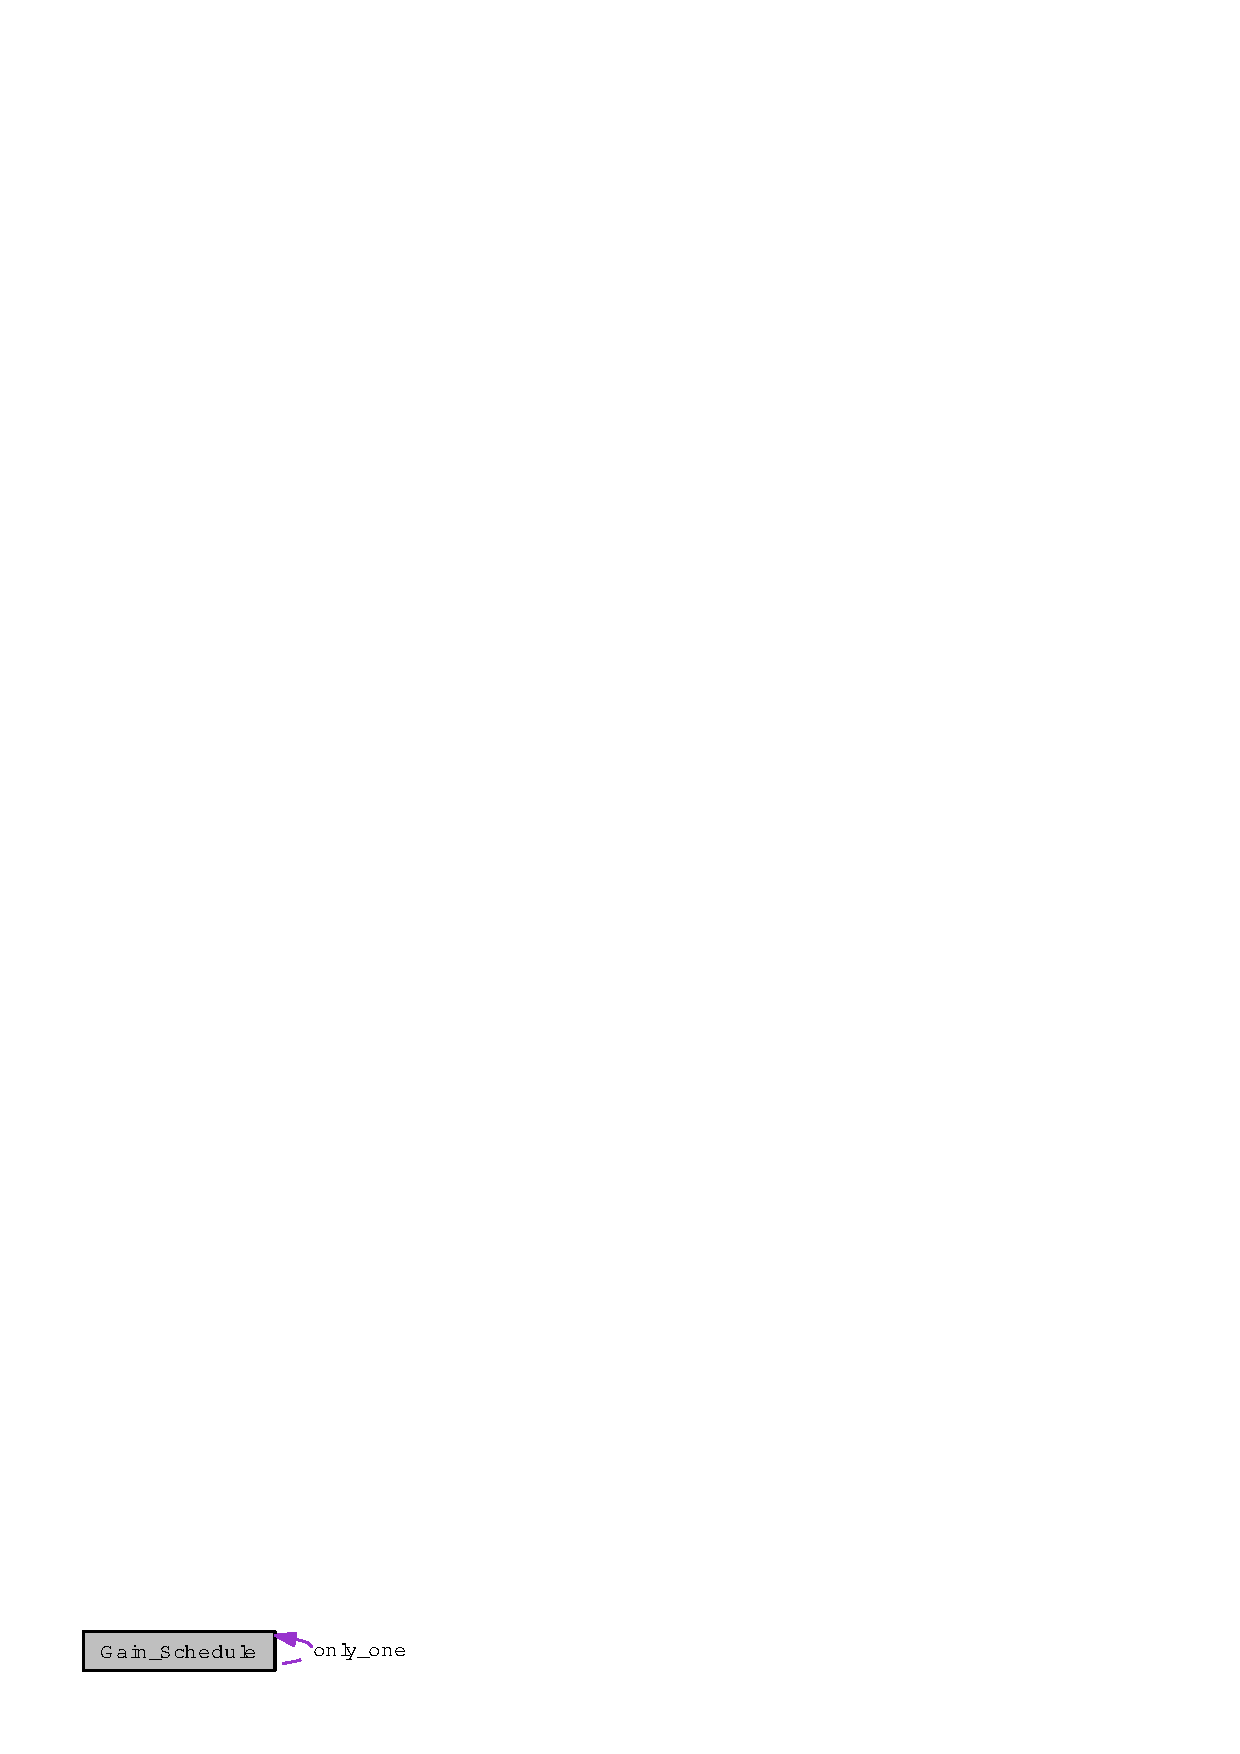
\includegraphics[width=100pt]{classGain__Schedule__coll__graph}
\end{center}
\end{figure}
\subsection*{Public Member Functions}
\begin{CompactItemize}
\item 
void {\bf update\-Max\-Gain} (void)
\item 
double {\bf get\-Max\-Gain} (void) const
\item 
double {\bf get\-Gain} (void) const
\item 
void {\bf reset\-Gain} (void)
\item 
void {\bf halve\-Gain} (void)
\end{CompactItemize}
\subsection*{Static Public Member Functions}
\begin{CompactItemize}
\item 
static {\bf Gain\_\-Schedule} \& {\bf instance} (void)
\end{CompactItemize}


\subsection{Member Function Documentation}
\index{Gain_Schedule@{Gain\_\-Schedule}!instance@{instance}}
\index{instance@{instance}!Gain_Schedule@{Gain\_\-Schedule}}
\subsubsection{\setlength{\rightskip}{0pt plus 5cm}{\bf Gain\_\-Schedule} \& Gain\_\-Schedule::instance (void)\hspace{0.3cm}{\tt  [static]}}\label{classGain__Schedule_e9eeedf767171cf65a3fa1ce7728a48d}


\index{Gain_Schedule@{Gain\_\-Schedule}!updateMaxGain@{updateMaxGain}}
\index{updateMaxGain@{updateMaxGain}!Gain_Schedule@{Gain\_\-Schedule}}
\subsubsection{\setlength{\rightskip}{0pt plus 5cm}void Gain\_\-Schedule::update\-Max\-Gain (void)}\label{classGain__Schedule_6cf994aea246dbfa7c0161a2ea85e8b7}


Update the maximum allowed value of gain and enforce limit. \index{Gain_Schedule@{Gain\_\-Schedule}!getMaxGain@{getMaxGain}}
\index{getMaxGain@{getMaxGain}!Gain_Schedule@{Gain\_\-Schedule}}
\subsubsection{\setlength{\rightskip}{0pt plus 5cm}double Gain\_\-Schedule::get\-Max\-Gain (void) const\hspace{0.3cm}{\tt  [inline]}}\label{classGain__Schedule_a48a7da15dfca933eaf64ff05effb27c}


Get max gain. \begin{Desc}
\item[Returns:]Maximum gain. \end{Desc}
\index{Gain_Schedule@{Gain\_\-Schedule}!getGain@{getGain}}
\index{getGain@{getGain}!Gain_Schedule@{Gain\_\-Schedule}}
\subsubsection{\setlength{\rightskip}{0pt plus 5cm}double Gain\_\-Schedule::get\-Gain (void) const\hspace{0.3cm}{\tt  [inline]}}\label{classGain__Schedule_c39682e959e22b2ce1a701aa11ab40ad}


Get gain. \begin{Desc}
\item[Returns:]Gain. \end{Desc}
\index{Gain_Schedule@{Gain\_\-Schedule}!resetGain@{resetGain}}
\index{resetGain@{resetGain}!Gain_Schedule@{Gain\_\-Schedule}}
\subsubsection{\setlength{\rightskip}{0pt plus 5cm}void Gain\_\-Schedule::reset\-Gain (void)\hspace{0.3cm}{\tt  [inline]}}\label{classGain__Schedule_75dcb2056c045ddaf16f3e72db0696ca}


Reset gain to reference value. /$\ast$$\ast$ Reset gain to max value. \index{Gain_Schedule@{Gain\_\-Schedule}!halveGain@{halveGain}}
\index{halveGain@{halveGain}!Gain_Schedule@{Gain\_\-Schedule}}
\subsubsection{\setlength{\rightskip}{0pt plus 5cm}void Gain\_\-Schedule::halve\-Gain (void)\hspace{0.3cm}{\tt  [inline]}}\label{classGain__Schedule_5fc79542643bd357116aea69735a1ac1}


Reduce gain by 50\%. 

The documentation for this class was generated from the following files:\begin{CompactItemize}
\item 
{\bf gain\_\-schedule.h}\item 
{\bf gain\_\-schedule.cc}\end{CompactItemize}
